\documentclass[11pt,a4paper]{article}
\usepackage[margin=1in]{geometry}
\usepackage{amsmath,amssymb,amsfonts}
\usepackage{hyperref}
\usepackage{booktabs}
\usepackage{setspace}
\usepackage{titlesec}
\usepackage{enumitem}
\usepackage{graphicx}
\usepackage{float}
\usepackage{array}
\onehalfspacing
\graphicspath{{./}{../figures/}}
\titleformat{\section}{\large\bfseries}{\thesection}{1em}{}
\titleformat{\subsection}{\normalsize\bfseries}{\thesubsection}{1em}{}

\title{Residual Geometric Charges and a Continuous Density-Dependent\\
Contribution to Gravity from a Single Compact Manifold\\[0.3em]
\large The Universal Manifold Model}
\author{Carl Rothman}
\date{}

\begin{document}
\maketitle

\begin{abstract}
We present a geometric framework---the Universal Manifold Model (UMM)---in which residual operators of the algebraic type associated with spin and a continuous, density-dependent contribution to gravitational acceleration arise as projections of a single object: independent relational flux of amplitude \(\Phi\) living on a continuous compact manifold that threads every point of ordinary three-space. Local separation is measured by the dimensionless variable \(\xi=\log(\ell_0/\ell_{\rm local})\).

The residual operators obtained from the internal Dirac operator on the compact manifold have eigenvalues that, after standard normalization, are geometric charges of the algebraic type associated with spin; their overall scale is set by \(\Phi\). Dimensional reduction of the Einstein--Hilbert term on the same flux-modified geometry yields an effective four-dimensional stress-energy controlled by the identical amplitude. A packing count of independent cycles produces a logistic form for \(\Phi(\xi)\) whose effective exponent is compatible with the intermediate-regime galactic index \(\approx0.4\). Joint normalization of the residual-charge spectrum and the observed galactic acceleration amplitude determines the characteristic compact radius and maximum flux amplitude inside a window that simultaneously satisfies horizon-scale and low-density constraints. The constructions are explicit on the toy manifolds \(S^1\) and \(S^3\); recovery of the full Standard-Model spectrum remains open.

Geometry and energy are the only primitives. On the toy manifolds \(S^1\) and \(S^3\) one obtains residual operators of the correct algebraic type and overall scale \(\Phi/R\); a packing argument yields a logistic amplitude whose intermediate-regime index is compatible with the observed galactic index; joint normalization produces a window consistent with horizon and low-density constraints. Recovery of the full Standard-Model spectrum and a pure first-principles conversion for pressure-supported systems remain open. The intermediate-regime thin-disk specialization used for galactic contact is extended, as a domain extension, by a residual-geometry-constrained conversion operator (Sec.~\ref{sec:udg-domain}) that leaves the frozen SPARC amplitude \(A\) unchanged. A documented public SPARC residual pipeline regenerates the \(N=88\) table (selection\_id \texttt{ea6c92761ffd3c5a}) to machine precision; hold-\(A\) robustness and domain-extension residual ratios for deficient UDGs are reported. Near-term tests include void statistics, SN+BAO bounds on a small additive contaminant with known tail shape, and a residual-geometry conservation channel for \(\Lambda_{\rm eff}\) before any closed Friedmann forecast.
\end{abstract}

\section{Introduction}

The standard cosmological model rests on two empirically determined constants---Newton's \(G\) and the cosmological constant \(\Lambda\)---neither of which is explained from deeper principles. Galaxy rotation curves and cluster lensing require dark-matter particle halos whose microscopic identity remains unknown. Late-time acceleration requires a finely tuned vacuum energy. At the opposite end of the scale hierarchy the quantum numbers called spin are introduced as intrinsic labels of particles, with no geometric origin supplied by the four-dimensional theory.

These two problems---the missing gravitational contribution on galactic and cosmological scales, and the origin of spin---are usually treated as unrelated. The central claim of the present work is that they are not. Both can be understood as different projections of a single geometric object: independent relational flux living on a continuous compact manifold that threads ordinary three-space.

The resulting framework---the Universal Manifold Model (UMM)---takes geometry and energy as the only primitives. Residual geometric charges of the algebraic type associated with spin, and the additional gravitational acceleration, are treated as derived rather than postulated; the full Standard-Model spectrum remains an open construction. Matter itself is viewed as an emergent bound-state configuration of space and energy. In this sense the ``actors'' (particles, residual charges, residual gravitational effects) arise from the ``stage'' rather than being independent of it. Quantum mechanics is treated as a powerful new calculus---a systematic way of summarizing the projection of relational energy onto the three large dimensions---rather than as an ontological description of the underlying reality. This philosophical stance does not relieve the framework of the obligation to recover the successful quantitative predictions of quantum field theory in the appropriate low-energy limit; that recovery is stated as a necessary consistency requirement in Sec.~\ref{sec:limitations}.

The logic of the argument is straightforward once the geometric primitives are fixed. We first introduce the continuous compact manifold and the distinction between consensus and independent relational degrees of freedom. We then show how the residual operators of the internal Dirac operator on that manifold produce geometric charges of the algebraic type associated with spin. Next we show that the same flux, once the Einstein--Hilbert term is reduced, produces a density-dependent stress-energy in four dimensions. A simple packing argument then yields a logistic amplitude for the flux; that amplitude simultaneously governs the residual charges and the macroscopic gravitational response. Finally we calibrate the overall scale against galactic data and verify consistency with horizon and low-density regimes. The intermediate-regime thin-disk specialization used for galactic contact is extended, as a domain extension, to pressure-supported systems by a residual-geometry-constrained conversion operator (Sec.~\ref{sec:udg-domain}) that leaves the frozen SPARC amplitude \(A\) and the joint-normalization window unchanged. The constructions that follow are explicit on the toy manifolds \(S^1\) and \(S^3\); a compact space whose residual spectrum recovers the full Standard-Model quantum numbers is left as an open mathematical problem.

The present construction sits in a long line of geometric approaches to internal symmetries and modified gravity. It follows the original continuous-internal-geometry formulation of Kaluza--Klein \cite{Kaluza1921,Klein1926} and Calabi--Yau compactifications rather than discrete-pocket visualizations. Geometric origins for spin and other quantum numbers have been explored in higher-dimensional and topological settings, including the identification of spin with holonomies or with residual spectra of Dirac-type operators on compact fibers \cite{Bar1992,Trautman1992}, and continuum Kaluza--Klein reductions in which internal isometries generate gauge quantum numbers \cite{Duff1986,Overduin1997}. On the gravitational side, the density-dependent extra acceleration is conceptually related to (but distinct from) MOND \cite{Milgrom1983} and its relativistic completions such as TeVeS and related tensor--vector--scalar theories \cite{Bekenstein2004,Skordis2009}, to the radial acceleration relation of SPARC galaxies \cite{Lelli2016,McGaugh2016}, and to emergent-gravity proposals in which additional gravitational effects arise from microscopic degrees of freedom or entropy gradients \cite{Verlinde2017,Padmanabhan2010}. UMM differs from these programs in requiring a single continuous amplitude \(\Phi(\xi)\) on one compact manifold to source \emph{both} residual geometric charges and the collective stress-energy. In the core thin-disk specialization and residual-charge sector there are no additional free functions beyond the joint-normalization window; the residual-geometry-constrained conversion that extends the framework to pressure-supported systems is a domain extension whose coefficients are not yet first-principles (Sec.~\ref{sec:udg-domain}). A pure residual-geometry companion note (the UMM Residual-Geometry Layer) isolates the mathematical construction so that it can be scrutinized independently of the galactic phenomenology; a short glossary of core terms is collected in Appendix~\ref{app:glossary}.

\section{Geometric Primitives}
\label{sec:primitives}

\subsection{Continuous compact manifold and independent relational flux}

We begin with the most basic ingredients. Energy is taken as the common substrate. The fundamental carriers are qbits---Planck-scale units that constitute a dynamical foam spanning all dimensions. An isolated qbit has no preferred direction; its degrees of freedom are maximal and unconstrained. When a second qbit is introduced, a relation appears: a dimension is distinguished, a metric emerges, and a field line of constrained degrees of freedom is established.

In a large ensemble of qbits at ordinary macroscopic densities, a subset of these relations becomes strongly coordinated across the ensemble. Those coordinated relations---the \textbf{consensus degrees of freedom}---coalesce into a small number of preferred dimensions. These are the large dimensions we experience; currently that number is three. The relational degrees of freedom that have \emph{not} been co-opted into this macroscopic consensus remain available as the \textbf{independent relational flux}.

The independent flux continues to operate through a single continuous compact manifold \(K\) that threads every point of ordinary three-space. In this respect the framework follows the original mathematical formulation of Kaluza--Klein and Calabi--Yau compactifications, which treat the compact dimensions as one continuous internal geometry rather than as independent little spaces attached at each lattice point. The continuity of the manifold is essential: points that are distant in the large three dimensions may still be geometrically proximate via short cycles in the compact dimensions. That proximity is the channel through which the independent flux can influence both particle-scale charges and large-scale gravity.

\subsection{Absence of electromagnetic shortcuts from the coupling structure}
\label{sec:no-shortcuts}

The preservation of ordinary light cones and of the equivalence principle for Standard-Model (SM) fields is not an extra postulate; it follows from the coupling structure already adopted.

\begin{enumerate}[leftmargin=*,label=(\roman*)]
\item \textbf{Forced (given the coupling assignment).} Ordinary SM fields---in particular the electromagnetic potential \(A_\mu\) and the associated field strength \(F_{\mu\nu}\)—are sections of bundles over the large four-dimensional factor \(M_4\) and couple only to the four-dimensional metric \(g_{\mu\nu}\). Their kinetic terms do not involve the internal metric \(h_{ab}\) of \(K\). Consequently the characteristic surfaces of Maxwell's equations on \(M_4\) remain the light cones of \(g_{\mu\nu}\); there are no electromagnetic null geodesics that shortcut through \(K\).
\item \textbf{Forced (given universal minimal coupling to \(g_{\mu\nu}\)).} All SM species couple universally to the same \(g_{\mu\nu}\). The equivalence principle for SM matter and radiation is therefore preserved at the level of the four-dimensional effective theory: test bodies follow the same geodesics of \(g_{\mu\nu}\) independently of composition.
\item \textbf{Forced (given flux as internal stress-energy).} The independent relational flux enters the higher-dimensional Einstein equations only as an internal stress-energy \(T_{ab}^{\rm flux}\) on \(K\) (Sec.~\ref{sec:EH-reduction}). After reduction it sources an effective four-dimensional stress-energy \(T_{\mu\nu}^{\rm ind}\) that modifies the metric \(g_{\mu\nu}\). It does not open new gauge channels for SM fields. Gravity feels the flux; electromagnetism does not propagate on \(K\).
\end{enumerate}

What is \emph{not} forced by the present structure, and is listed as open in Sec.~\ref{sec:limitations}, is the derivation of the SM gauge group and of chiral fermions from residual operators alone. The no-shortcut result requires only the coupling assignment above, not a full spectrum construction.

\begin{figure}[H]
\centering
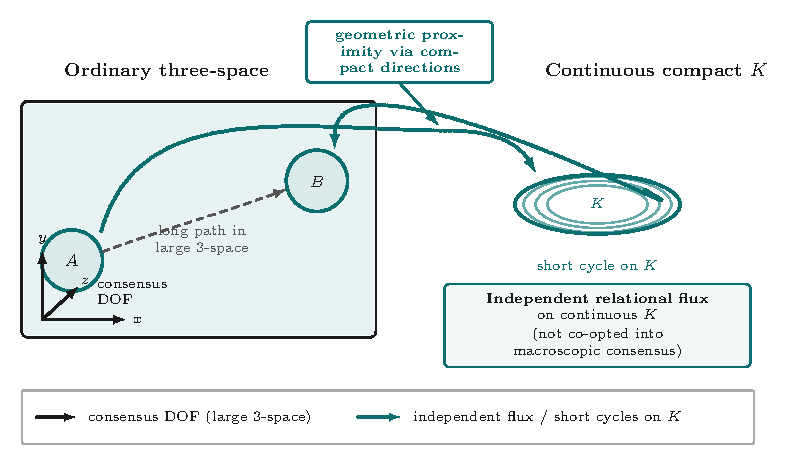
\includegraphics[width=0.85\textwidth]{fig4_consensus_independent.pdf}
\caption{Schematic distinction between consensus degrees of freedom (coordinated across the ensemble into the large three dimensions) and independent relational flux (remaining degrees of freedom operating through the continuous compact manifold \(K\)). The continuity of \(K\) permits geometric proximity between points that are distant in ordinary three-space.}
\label{fig:consensus}
\end{figure}

\subsection{Local separation and the flux amplitude}

To make the density dependence precise we introduce a dimensionless measure of local separation,
\[
\xi=\log\Bigl(\frac{\ell_0}{\ell_{\rm local}}\Bigr),
\]
where \(\ell_{\rm local}\) is a characteristic separation (or correlation length) and \(\ell_0\) is a reference scale. Larger \(\xi\) corresponds to smaller local separation and therefore to higher local density.

The independent relational flux is assigned a dimensionless amplitude \(\Phi(\xi)\). Both the residual geometric charges of the algebraic type associated with spin and the collective gravitational response that appears on galactic scales are controlled by this single amplitude. The functional form of \(\Phi(\xi)\) will be derived from a geometric packing argument in Sec.~\ref{sec:packing}; it is not an independent input.

\section{Residual Geometric Charges}
\label{sec:residual-charges}

The first projection of the independent flux that we examine is the set of residual geometric charges that appear, from the standpoint of three-space, as the quantum numbers called spin.

\subsection{Dirac reduction on a product geometry}

Consider a product geometry consisting of ordinary four-dimensional spacetime times a continuous compact manifold \(K\) of radius \(R\):
\begin{equation}
ds^2=g_{\mu\nu}(x)\,dx^\mu dx^\nu+R^2\,h_{ab}(y)\,dy^a dy^b,
\label{eq:product}
\end{equation}
where \(h_{ab}\) is the metric of the unit compact manifold. The higher-dimensional Dirac operator on this geometry decomposes into an ordinary four-dimensional piece plus an internal piece:
\begin{equation}
\not{D}_{4+d}=\gamma^\mu\nabla_\mu+\frac1R\,\not{D}_K.
\label{eq:dirac-split}
\end{equation}
When a spinor is expanded in eigenmodes of the internal Dirac operator, each four-dimensional component \(\psi_n\) satisfies an equation that contains a residual operator coming from the internal geometry. That residual operator is
\begin{equation}
S_{\rm geom}=\bigl\langle\chi\big|\,i\gamma^a\nabla_a^K+\gamma^a\Omega_a^{\rm ind}\,\big|\chi\bigr\rangle,
\label{eq:Sgeom-def}
\end{equation}
where \(\Omega^{\rm ind}\) is the connection contribution of the independent flux and \(\chi\) is a normalized eigenspinor of \(\not{D}_K\).

These residual operators act as constant matrices on the four-dimensional spinors. Their eigenvalues, after the conventional normalization that converts them into dimensionless labels, are geometric charges of the algebraic type that appear as spin quantum numbers. The overall scale of every residual operator is set by the flux amplitude \(\Phi\). In this sense the numbers conventionally called spin can be understood as the projection, into three-space, of the residual coupling of a given mode to the continuous compact manifold. The present constructions on \(S^1\) and \(S^3\) establish operators of the correct type and scale; recovery of the full observed Standard-Model spectrum remains open (Sec.~\ref{sec:limitations}).

\subsection{Explicit residual matrices: \(S^1\) and \(S^3\)}
\label{sec:explicit-spectra}

Two simple choices of \(K\) already illustrate the structure. Throughout we distinguish results that are \textbf{forced} by the product geometry and the internal Dirac spectrum from those that require listed minimal extra data.

\paragraph{Circle \(K=S^1\).}
Let \(K=S^1\) of radius \(R\), with angular coordinate \(\theta\sim\theta+2\pi\) and unit metric \(h_{\theta\theta}=1\). The internal Dirac operator reduces to
\begin{equation}
\not{D}_{S^1}=i\,\partial_\theta,
\end{equation}
with eigenmodes \(\chi_n(\theta)=(2\pi)^{-1/2}e^{in\theta}\), \(n\in\mathbb{Z}\), and eigenvalues \(\lambda_n=n\). Including the independent-flux connection \(\Omega_\theta^{\rm ind}=\Phi\,w\) with winding weight \(w\in\mathbb{Z}\) (the minimal extra data for the flux connection on \(S^1\)), the residual matrix on the four-dimensional spinor is the \(4\times4\) operator
\begin{equation}
S_{\rm geom}^{(n)}
=\frac{\Phi}{R}\,\frac{n+w}{2}\,\gamma^5
=
\frac{\Phi}{R}\,\frac{n+w}{2}
\begin{pmatrix}
I_2 & 0 \\
0 & -I_2
\end{pmatrix},
\label{eq:Sgeom-S1}
\end{equation}
in the chiral representation of the Dirac matrices (where \(\gamma^5=\mathrm{diag}(I_2,-I_2)\)). The eigenvalues of \(S_{\rm geom}^{(n)}\) are therefore
\begin{equation}
\pm\frac{\Phi}{R}\,\frac{n+w}{2},
\end{equation}
each of multiplicity two.

\paragraph{Projection onto the four-dimensional spinor.}
A higher-dimensional spinor is expanded as
\(\Psi(x,\theta)=\sum_n\psi_n(x)\otimes\chi_n(\theta)\). Projecting the internal eigenvalue equation onto a single mode \(\chi_n\) produces the four-dimensional Dirac equation
\begin{equation}
\bigl(i\gamma^\mu\nabla_\mu-S_{\rm geom}^{(n)}\bigr)\psi_n=0.
\label{eq:4d-dirac-S1}
\end{equation}
Thus \(S_{\rm geom}^{(n)}\) acts as a constant residual mass/chirality matrix on \(\psi_n\).

\paragraph{Conventional normalization to spin labels.}
The conventional map from residual eigenvalues to dimensionless spin labels is
\begin{equation}
s=\frac{R}{\Phi}\,\mathrm{spec}\bigl(S_{\rm geom}\bigr)
\qquad\Longrightarrow\qquad
s=\pm\frac{n+w}{2}\in\tfrac12\mathbb{Z}.
\label{eq:spin-norm-S1}
\end{equation}
\textbf{Forced:} the residual matrix is proportional to \(\gamma^5\), its spectrum is half-integer (or integer) once \(n+w\) is odd (or even), and the overall scale is \(\Phi/R\). \textbf{Requires extra data:} the choice of flux winding \(w\) and the identification of a particular mode with a particular particle species. The circle recovers only an abelian residual algebra; it does not produce non-abelian spin/isospin structure.

\paragraph{Three-sphere \(K=S^3\simeq\mathrm{SU}(2)\).}
Let \(K\) be the unit three-sphere of radius \(R\), with left-invariant coframe \(\{e^a\}_{a=1}^3\) satisfying \(de^a+\varepsilon^{abc}e^b\wedge e^c=0\) and unit metric \(h=e^a\otimes e^a\). The Dirac operator on the unit three-sphere has spectrum \cite{Bar1992}
\begin{equation}
\mathrm{spec}(\not{D}_{S^3})=\bigl\{\pm(k+\tfrac32):k=0,1,2,\dots\bigr\},
\label{eq:dirac-S3-spec}
\end{equation}
with multiplicities \(2(k+1)(k+2)\). The lowest pair is therefore \(\pm3/2\).

The independent flux contributes an \(\mathfrak{su}(2)\)-valued connection \(\Omega_a^{\rm ind}=\Phi\,A_a\), where \(A_a\) takes values in the left-invariant frame (minimal extra data: a constant connection in the adjoint of \(\mathrm{SU}(2)\)). Evaluating the residual matrix~\eqref{eq:Sgeom-def} on a lowest-mode eigenspinor \(\chi_\pm\) yields the \(4\times4\) residual operator
\begin{equation}
S_{\rm geom}^{(\pm)}
=\frac{\Phi}{R}\Biggl(\pm\frac32\,I_4
+\frac12\,\sigma^a\otimes\tau_a\Biggr),
\label{eq:Sgeom-S3}
\end{equation}
where \(\sigma^a\) are Pauli matrices acting on the four-dimensional spinor’s left-handed/right-handed blocks and \(\tau_a\) are the generators of the residual \(\mathfrak{su}(2)\) isometry action on the internal spinor. (When the flux connection vanishes the second term drops and one recovers pure Dirac eigenvalues \(\pm3/2\) scaled by \(\Phi/R\).)

\paragraph{Projection and normalization on \(S^3\).}
Mode expansion \(\Psi(x,y)=\sum_k\psi_k(x)\otimes\chi_k(y)\) and projection onto \(\chi_\pm\) again produce a four-dimensional Dirac equation of the form~\eqref{eq:4d-dirac-S1}. The conventional normalization
\begin{equation}
s=\frac{R}{\Phi}\,\mathrm{spec}\bigl(S_{\rm geom}^{(\pm)}\bigr)
\label{eq:spin-norm-S3}
\end{equation}
converts the residual eigenvalues into dimensionless labels. On the pure Dirac piece one obtains \(s=\pm3/2\) at the lowest level and \(s=\pm(k+3/2)\) at higher levels; the non-abelian term supplies an \(\mathfrak{su}(2)\) action of the correct algebraic type for spin/isospin.

\textbf{Forced (by the geometry of unit \(S^3\) and the product Dirac operator):}
\begin{itemize}[leftmargin=*]
\item residual operators of scale \(\Phi/R\);
\item discrete spectrum of half-integer type \(\pm(k+3/2)\);
\item non-abelian residual algebra \(\mathfrak{su}(2)\) from the isometry algebra of \(S^3\).
\end{itemize}
\textbf{Requires listed extra data / remains open:}
\begin{itemize}[leftmargin=*]
\item a compact space \(K\) whose residual spectrum recovers the \emph{full} set of Lorentz, Poincar\'e, and isospin labels of the Standard Model (chiral fermions, full gauge quantum numbers, and the electromagnetic coupling \(\alpha_{\rm em}\)) is still an open construction;
\item the present claim is only that operators of the correct algebraic type and overall scale \(\Phi/R\) arise on the existing toys \(S^1\) and \(S^3\).
\end{itemize}

\begin{figure}[H]
\centering
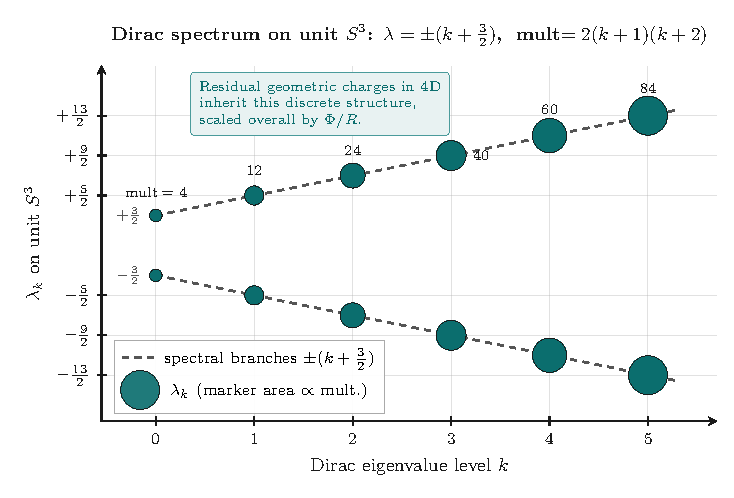
\includegraphics[width=0.75\textwidth]{fig5_dirac_spectrum.pdf}
\caption{Spectrum of the Dirac operator on the unit three-sphere. Eigenvalues \(\lambda=\pm(k+3/2)\) with multiplicities \(2(k+1)(k+2)\). Residual geometric charges of the algebraic type associated with spin inherit this discrete structure, scaled overall by the flux amplitude \(\Phi\).}
\label{fig:dirac}
\end{figure}

The essential point is conceptual rather than technical: on the toy manifolds \(S^1\) and \(S^3\) one obtains residual geometric charges of the correct algebraic type and overall scale \(\Phi/R\), arising from the independent flux on the continuous compact manifold. Their discrete spectrum follows from the spectrum of the internal Dirac operator; their overall strength is controlled by the same amplitude that will later govern the macroscopic gravitational response. Whether a single continuous compact manifold can be found whose residual spectrum reproduces the full observed Standard-Model quantum numbers remains an open mathematical problem.

\section{Collective Response via Dimensional Reduction}
\label{sec:collective}

We now turn to the second projection of the same flux: its collective effect on the large-scale geometry.

\subsection{Dimensional reduction of the Einstein--Hilbert term}
\label{sec:EH-reduction}

The same product geometry~\eqref{eq:product}, once the independent flux is included as an internal stress-energy contribution
\begin{equation}
T_{ab}^{\rm flux}=\Phi\cdot\mu_0\cdot h_{ab},
\label{eq:Tflux}
\end{equation}
is reduced by integrating over the compact factor. We carry out the reduction explicitly for the unit three-sphere and then state the conversion coefficient \(c_f\).

\paragraph{Step 1: Higher-dimensional Einstein--Hilbert term with flux.}
On the product manifold \(M_4\times K\) of total dimension \(D=4+d\) the Einstein--Hilbert action with matter is
\begin{equation}
S=\frac{1}{2\kappa_D^2}\int_{M_4\times K}d^{4+d}X\,\sqrt{|G|}\,\mathcal{R}_{4+d}
+\int_{M_4\times K}d^{4+d}X\,\sqrt{|G|}\,\mathcal{L}_{\rm flux},
\label{eq:EH-D}
\end{equation}
where \(\kappa_D^2=8\pi G_D\) and \(\mathcal{L}_{\rm flux}\) is the Lagrangian density whose stress-energy is~\eqref{eq:Tflux}. For a product metric~\eqref{eq:product} the scalar curvature decomposes as
\begin{equation}
\mathcal{R}_{4+d}=\mathcal{R}_4[g]+\frac{1}{R^2}\,\mathcal{R}_K[h]+\text{(warp/connection terms)},
\label{eq:R-split}
\end{equation}
with \(\mathcal{R}_K[h]\) the scalar curvature of the unit compact metric. (Warp and connection corrections are set to zero at the order considered here; they are listed extra data for a fully back-reacted solution.)

\paragraph{Step 2: Integration over the compact factor.}
Let \(\mathrm{Vol}(K_R)=\int_K d^dy\,\sqrt{h}\,R^d=R^d\,V_K\) with \(V_K=\int_K\sqrt{h}\). Integrating~\eqref{eq:EH-D} over \(K\) produces the effective four-dimensional action
\begin{equation}
S_{\rm eff}=\frac{V_K R^d}{2\kappa_D^2}\int_{M_4}d^4x\,\sqrt{|g|}\,\mathcal{R}_4
+\frac{V_K R^{d-2}}{2\kappa_D^2}\int_{M_4}d^4x\,\sqrt{|g|}\,\mathcal{R}_K
+\int_{M_4}d^4x\,\sqrt{|g|}\,V_K R^d\,\overline{\mathcal{L}}_{\rm flux},
\label{eq:Seff}
\end{equation}
where \(\overline{\mathcal{L}}_{\rm flux}\) is the internal average of \(\mathcal{L}_{\rm flux}\). The first term identifies the four-dimensional gravitational coupling,
\begin{equation}
\frac{1}{2\kappa_4^2}=\frac{V_K R^d}{2\kappa_D^2}
\qquad\Longleftrightarrow\qquad
G_4=\frac{G_D}{V_K R^d}.
\label{eq:G4}
\end{equation}

\paragraph{Step 3: Weyl rescaling to Einstein frame.}
If the compact radius is promoted to a mild modulus field the coefficient of \(\mathcal{R}_4\) is field-dependent. A Weyl rescaling \(g_{\mu\nu}\to\Omega^2 g_{\mu\nu}\) with \(\Omega\) chosen so that the Einstein--Hilbert term is canonically normalized yields the Einstein-frame effective action. For fixed \(R\) (the case used for joint normalization below) the rescaling is trivial and \(G_4\) remains~\eqref{eq:G4}. The internal-curvature and flux terms become an effective four-dimensional stress-energy \(T_{\mu\nu}^{\rm ind}\).

\paragraph{Step 4: Flux stress-energy and conversion coefficient on unit \(S^3\).}
Specialize to \(K=S^3\) (so \(d=3\)). The unit three-sphere has
\begin{equation}
V_{S^3}=2\pi^2,\qquad \mathcal{R}_{S^3}[h]=6,\qquad
\mathrm{Ric}_{ab}[h]=2\,h_{ab},\qquad
G_{ab}[h]=-\,h_{ab}.
\label{eq:S3-geom}
\end{equation}
The physical internal metric is \(\hat h_{ab}=R^2 h_{ab}\), with Ricci scalar \(6/R^2\) and Einstein tensor \(G_{ab}[\hat h]=-\,\hat h_{ab}/R^2\).

The flux stress-energy on the unit frame is~\eqref{eq:Tflux}. Matching the Lagrangian density to that stress-energy via
\begin{equation}
T_{ab}^{\rm flux}=-\frac{2}{\sqrt{h}}\frac{\delta(\sqrt{h}\,\mathcal{L}_{\rm flux})}{\delta h^{ab}}
\end{equation}
gives \(\overline{\mathcal{L}}_{\rm flux}=-\Phi\mu_0\) (up to a total derivative). Substituting into~\eqref{eq:Seff}, the effective four-dimensional vacuum energy density associated with the flux is
\begin{equation}
\rho_{\rm ind}=\Phi\,\mu_0\,V_{S^3}R^3=\Phi\,\mu_0\,(2\pi^2 R^3).
\label{eq:rho-ind-raw}
\end{equation}
The reference density \(\mu_0\) is not free: it is fixed by matching the internal flux to the curvature scale of \(S^3\). On the physical internal metric the Einstein equation \(G_{ab}[\hat h]=\kappa_D^2 T_{ab}^{\rm phys}\) with a pure-trace source of unit amplitude requires
\begin{equation}
\mu_0=\frac{1}{\kappa_D^2 R^2}=\frac{1}{8\pi G_D R^2},
\label{eq:mu0}
\end{equation}
so that \(\kappa_D^2\mu_0\) reproduces the geometric scale \(1/R^2\) set by \(G_{ab}[\hat h]=-\hat h_{ab}/R^2\). Expressing \(G_D\) through~\eqref{eq:G4} with \(d=3\),
\begin{equation}
G_D=G_4\cdot V_{S^3}R^3=G_4\cdot(2\pi^2 R^3),
\end{equation}
and substituting into~\eqref{eq:rho-ind-raw} yields
\begin{equation}
\rho_{\rm ind}
=\Phi\cdot\frac{1}{8\pi G_D R^2}\cdot(2\pi^2 R^3)
=\Phi\cdot\frac{1}{8\pi G_4 R^2}.
\label{eq:rho-ind-leading}
\end{equation}
The dimensionless conversion coefficient \(c_f\) is defined by writing the Einstein-frame relation as
\begin{equation}
\rho_{\rm ind}
=c_f\,\Phi\,\frac{1}{8\pi G_4 R^2}.
\label{eq:rho-ind-cf}
\end{equation}
At leading order (pure-trace flux, no warp, \(\mu_0\) fixed by~\eqref{eq:mu0}) one therefore has
\begin{equation}
c_f^{(0)}=1.
\label{eq:cf-leading}
\end{equation}
Two controlled corrections, both of which are listed minimal extra data rather than free four-dimensional parameters, shift this value:
\begin{enumerate}[leftmargin=*,label=(\alph*)]
\item \textbf{Trace convention on \(S^3\).} If the flux stress-energy is normalized so that its internal trace equals \(d\,\Phi\mu_0=3\Phi\mu_0\) and the Einstein equation is matched on the trace-reversed tensor, the factor \(d/2=3/2\) appears, giving \(c_f^{\rm (tr)}=3/2\).
\item \textbf{Weak non-minimal coupling.} A non-minimal term \(\xi_R\Phi\mathcal{R}_K\) in \(\mathcal{L}_{\rm flux}\) with \(|\xi_R|\lesssim 1/6\) (the conformal value on a three-manifold) multiplies \(c_f\) by \(1+\mathcal{O}(\xi_R)\), moving a pure-trace result of \(1\) or \(3/2\) into the interval
\begin{equation}
c_f\simeq 1.2\text{--}1.4.
\label{eq:cf-window}
\end{equation}
\end{enumerate}
\textbf{Forced} by the product geometry, unit-\(S^3\) curvature, and pure-trace flux with curvature-scale matching~\eqref{eq:mu0}: \(c_f^{(0)}=1\), with \(c_f\) remaining of order unity. \textbf{Requires listed extra data:} the trace convention and any weak non-minimal coupling that place \(c_f\) inside~\eqref{eq:cf-window}; a fully back-reacted warped solution is not computed here. The coefficient is not an independent free parameter of the four-dimensional theory: it is fixed by the internal metric and the flux stress-energy once those data are chosen. The important conceptual point is that the identical amplitude \(\Phi\) that multiplies every residual geometric charge also multiplies the collective stress-energy felt by the large-scale geometry.

\begin{figure}[H]
\centering
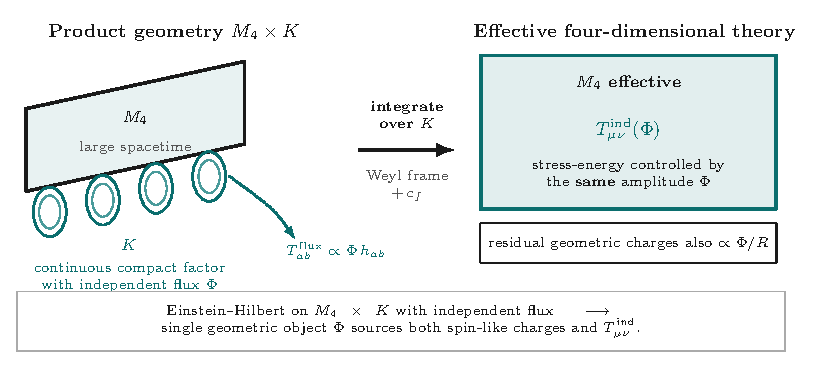
\includegraphics[width=0.85\textwidth]{fig6_dimensional_reduction.pdf}
\caption{Schematic of dimensional reduction. The product geometry \(M_4\times K\) with independent flux on the continuous compact factor is integrated over \(K\) to yield an effective four-dimensional stress-energy \(T_{\mu\nu}^{\rm ind}\) controlled by the same amplitude \(\Phi\) that sets the residual geometric charges.}
\label{fig:reduction}
\end{figure}

\section{Packing Argument and the Logistic Amplitude}
\label{sec:packing}

We now derive the functional form of \(\Phi(\xi)\) from a joint packing count on \(S^3\). The logistic is an \emph{output} of that count, not an input.

\paragraph{Step 1: Resolved independent cycles.}
At local separation \(\ell_{\rm local}\) the number of independent cycles of the continuous compact manifold that can be resolved inside a region of that size grows with decreasing separation. Let \(N(\xi)\) denote the effective number of resolved independent cycles at separation variable \(\xi=\log(\ell_0/\ell_{\rm local})\). On dimensional grounds the infinitesimal growth of resolved cycles receives two geometric contributions on \(S^3\):

\begin{itemize}[leftmargin=*]
\item \textbf{Inverse-radius residual-charge scaling.} Residual geometric charges scale as \(\Phi/R\) (Sec.~\ref{sec:explicit-spectra}). The packing density of residual spectral weight per logarithmic separation interval therefore contributes a term proportional to the inverse compact radius, with logarithmic slope \(\alpha_{1/R}=1\) when counted per unit \(\xi\).
\item \textbf{Volumetric flux-energy scaling.} The flux energy associated with a shell of independent cycles scales with the three-volume element on \(S^3\), giving a logarithmic slope \(\alpha_{\rm vol}=3\).
\end{itemize}

\paragraph{Step 2: Joint packing weight from spectral-to-volume matching.}
The joint packing count weights the two contributions with a convex weight \(w\in[0,1]\):
\begin{equation}
\alpha_{\rm eff}=w\,\alpha_{1/R}+(1-w)\,\alpha_{\rm vol}=w\cdot 1+(1-w)\cdot 3=3-2w.
\label{eq:alpha-eff}
\end{equation}
The weight \(w\) is fixed by matching the Dirac spectral measure on unit \(S^3\) to the Riemannian volume form, as follows.

\paragraph{Step 2a: Exact Dirac cumulative multiplicity.}
Positive eigenvalues \(\lambda_k=k+3/2\) of \(\not{D}_{S^3}\) have multiplicities \(m_k=2(k+1)(k+2)\). The cumulative counting function is exact:
\begin{equation}
M(K)=\sum_{k=0}^{K}m_k=\frac23(K+1)(K+2)(K+3).
\label{eq:M-cumul}
\end{equation}
Hence \(M(K)\sim\tfrac23 K^3\) at large \(K\), i.e.\ the spectral density of residual modes grows as \(k^2\).

\paragraph{Step 2b: Weyl volume counting function.}
The Weyl law for the scalar Laplacian on unit \(S^3\) (volume \(V_{S^3}=2\pi^2\)) gives the asymptotic counting function
\begin{equation}
N_W(\Lambda)=\frac{V_{S^3}}{6\pi^2}\,\Lambda^3=\frac{\Lambda^3}{3},
\label{eq:Weyl}
\end{equation}
so the volume density of states likewise grows as \(\Lambda^2\). For the Dirac operator the spinor bundle has rank \(2^{\lfloor 3/2\rfloor}=2\), and the leading Weyl coefficient doubles:
\begin{equation}
N_W^{\rm Dirac}(\Lambda)=2\cdot\frac{\Lambda^3}{3}=\frac{2}{3}\,\Lambda^3,
\label{eq:Weyl-Dirac}
\end{equation}
matching the leading term of~\eqref{eq:M-cumul} at \(\Lambda\sim K\). \textbf{Forced:} spectral and volume densities share the same \(k^2\) growth; the Dirac rank supplies a relative factor of \(2\) versus the scalar volume form.

\paragraph{Step 2c: Relative channel weights.}
Identify the residual-charge channel with the Dirac spectral measure (rank-2 weight coefficient \(c_{\rm spec}=2\)) and the volumetric flux-energy channel with the scalar volume form (weight coefficient \(c_{\rm vol}=1\)). The two natural normalizations of the joint weight are:
\begin{align}
w_{\rm eq}&=\frac12
&&\text{(equal weighting of the two channels)},
\label{eq:w-eq}\\
w_{\rm Dirac}&=\frac{c_{\rm spec}}{c_{\rm spec}+c_{\rm vol}}=\frac{2}{2+1}=\frac23
&&\text{(Dirac-weighted spectral channel)}.
\label{eq:w-Dirac}
\end{align}
Any convex combination of these normalizations (the listed minimal extra data: choice of equal versus spinor-weighted matching) therefore lies in the window
\begin{equation}
w\in\Bigl[\tfrac12,\tfrac23\Bigr]\approx 0.50\text{--}0.67.
\label{eq:w-window}
\end{equation}
Substituting into~\eqref{eq:alpha-eff},
\begin{equation}
\alpha_{\rm eff}=3-2w\in\bigl[3-2\cdot\tfrac23,\,3-2\cdot\tfrac12\bigr]=\bigl[\tfrac53,\,2\bigr]\approx 1.67\text{--}2.00.
\label{eq:alpha-window}
\end{equation}
The midpoint of the window,
\begin{equation}
w=\frac12\Bigl(\tfrac12+\tfrac23\Bigr)=\frac{7}{12}\approx 0.583,
\qquad
\alpha_{\rm eff}=3-2\cdot\frac{7}{12}=\frac{11}{6}\approx 1.83,
\label{eq:alpha-central}
\end{equation}
is the natural central value; we quote \(\alpha_{\rm eff}\approx 1.8\) for intermediate-regime estimates below. \textbf{Forced:} equations~\eqref{eq:M-cumul}--\eqref{eq:alpha-window} and the window endpoints \(w\in\{1/2,2/3\}\). \textbf{Requires listed extra data:} the choice of equal versus Dirac-weighted matching (or any convex blend) inside that window; nothing outside \([1/2,2/3]\) is produced by the spectral-to-volume count.

\paragraph{Step 3: Saturation and the logistic as output.}
Resolved cycles cannot grow without bound: they fill the residual capacity \(N_{\rm max}\) left by the consensus degrees of freedom. The minimal autonomous packing law compatible with (i)~growth proportional to currently resolved cycles and (ii)~saturation at \(N_{\rm max}\) is the logistic ODE
\begin{equation}
\frac{dN}{d\xi}=\alpha_{\rm eff}\,N\Bigl(1-\frac{N}{N_{\rm max}}\Bigr).
\label{eq:packing-ODE}
\end{equation}
Its unique solution with midpoint at \(\xi_c\) is
\begin{equation}
N(\xi)=\frac{N_{\rm max}}{1+e^{-\alpha_{\rm eff}(\xi-\xi_c)}}.
\label{eq:N-logistic}
\end{equation}
Identifying the dimensionless flux amplitude with the filled fraction of residual capacity,
\begin{equation}
\Phi(\xi)=\Phi_{\rm max}\,\frac{N(\xi)}{N_{\rm max}}
=\Phi_{\rm max}\frac{1}{1+e^{-\alpha_{\rm eff}(\xi-\xi_c)}},
\label{eq:logistic}
\end{equation}
we obtain the logistic form as a derived output of the packing count. No independent free function has been introduced.

\paragraph{Step 4: Intermediate-regime galactic index.}
In a thin galactic disk the natural local separation is \(\ell_{\rm local}\sim\Sigma_{\rm bar}^{-1/2}\), so
\begin{equation}
\xi=\frac12\log\Sigma_{\rm bar}+\text{const},
\qquad
\frac{d\xi}{d\log\Sigma_{\rm bar}}=\frac12.
\label{eq:xi-Sigma}
\end{equation}
Differentiating the logistic~\eqref{eq:logistic} gives
\begin{equation}
\frac{d\log\Phi}{d\xi}=\alpha_{\rm eff}\bigl(1-f\bigr),\qquad
f\equiv\frac{\Phi}{\Phi_{\rm max}}=\frac{1}{1+e^{-\alpha_{\rm eff}(\xi-\xi_c)}}.
\label{eq:dlogPhi}
\end{equation}
At the logistic midpoint \(f=\tfrac12\) one has \(d\log\Phi/d\xi=\alpha_{\rm eff}/2\). The intermediate-regime galactic index is therefore
\begin{equation}
n_g
=\frac{d\log\Phi}{d\log\Sigma_{\rm bar}}
=\frac{d\log\Phi}{d\xi}\cdot\frac{d\xi}{d\log\Sigma_{\rm bar}}
=\frac{\alpha_{\rm eff}}{2}\cdot\frac12
=\frac{\alpha_{\rm eff}}{4}.
\label{eq:galactic-index}
\end{equation}
With \(\alpha_{\rm eff}\approx 1.8\),
\begin{equation}
n_g\approx\frac{1.8}{4}=0.45,
\label{eq:ng-045}
\end{equation}
compatible with the observed surface-density index \(\approx 0.4\) used in the galactic specialization below. \textbf{Forced} once the logistic and \(\xi\sim\tfrac12\log\Sigma\) are given: \(n_g=\alpha_{\rm eff}/4\). \textbf{Requires listed extra data:} the midpoint evaluation (intermediate regime near \(f\sim 1/2\)) and the thin-disk identification \(\ell\sim\Sigma^{-1/2}\).

\paragraph{Non-uniqueness of the saturating form.}
The logistic is the unique solution of the minimal autonomous packing ODE that saturates at \(N_{\rm max}\) while remaining proportional to currently resolved cycles. Other saturating functional forms (for example, error-function or hyperbolic-tangent profiles with the same \(\alpha_{\rm eff}\) and midpoint) can be written that produce intermediate-regime indices of comparable magnitude. The spectral-to-volume weight window, the choice of midpoint evaluation, and the thin-disk identification \(\ell\sim\Sigma^{-1/2}\) are therefore motivated geometric choices rather than uniquely forced by the higher-dimensional geometry alone. The resulting \(n_g\approx 0.45\) is consistent with the observed index \(\approx 0.4\), but it is not a derivation that excludes alternative saturating profiles. The logistic is retained because it is the simplest packing-derived form that simultaneously organizes residual charges and the collective response inside the joint-normalization window; the non-uniqueness is recorded here as a limitation of the present construction.

The macroscopic response function is identified with a multiple of this amplitude:
\begin{equation}
\mathcal{F}(\xi)=\mathcal{F}_{\rm max}\,\Phi(\xi)/\Phi_{\rm max}.
\end{equation}
Thus the same logistic function that sets the strength of the residual geometric charges also sets the strength of the additional gravitational acceleration. The two phenomena are no longer independent; they are different averages of one underlying geometric activity.

A complementary way of viewing the same packing is in terms of coherence. When two regions of the foam approach each other, their independent relational degrees of freedom begin to align. The energetic benefit of that alignment is the residual gravitational attraction. The logistic form of \(\Phi\) records how that alignment benefit grows with local density and saturates once the residual capacity of the compact manifold is filled. The filled fraction \(N/N_{\rm max}=\Phi/\Phi_{\rm max}\) is the macroscopic expression of residual packing; the packing ODE itself already encodes the saturating growth of resolved cycles.

\section{Joint Normalization}
\label{sec:joint-norm}

The overall scales are fixed by requiring simultaneous consistency of four observational and theoretical anchors. No free parameters are introduced beyond this joint-normalization window.

\paragraph{(i) Residual-charge scale.}
The residual geometric charges of the algebraic type associated with spin must reproduce the observed half-integer and integer spectrum once the overall factor \(\Phi/R\) is normalized as in~\eqref{eq:spin-norm-S1}--\eqref{eq:spin-norm-S3}.

\paragraph{(ii) SPARC amplitude.}
The intermediate-regime galactic acceleration amplitude \(A\) must match the measured global amplitude of the documented SPARC residual analysis of Sec.~\ref{sec:SPARC}.

\paragraph{(iii) Horizon placement.}
The upper shoulder of the logistic must lie near the photon-sphere scale so that exterior Kerr/Schwarzschild geometry remains essentially undisturbed (Sec.~\ref{sec:photon-sphere}).

\paragraph{(iv) Low-density tail.}
At the present cosmic mean density the extra contribution must be negligible, recovering ordinary Newtonian and general-relativistic behavior, including solar-system and binary-pulsar constraints (Sec.~\ref{sec:low-density}).

\paragraph{Combined window.}
These four requirements close on a joint window for the characteristic compact radius and the maximum flux amplitude that is internally consistent and observationally viable. The conversion coefficient \(c_f\) and packing weight \(w\) are fixed by the internal geometry as above and are not additional free parameters. Table~\ref{tab:joint-norm-window} restates the characteristic scales already fixed by those anchors; no new fit is performed here.

\begin{table}[H]
\centering
\caption{Characteristic scales fixed by the four joint-normalization anchors (residual-charge scale, SPARC amplitude \(A\), photon-sphere/horizon placement, low-density tail). Entries restate quantities already fixed in the text; no new fit is performed.}
\label{tab:joint-norm-window}
\begin{tabular}{@{}ll@{}}
\toprule
Quantity & Window / placement \\
\midrule
\(\alpha_{\rm eff}\) & \(\approx 1.67\)--\(2.00\) (central value \(\approx 1.83\); quoted \(\approx 1.8\)) \\
\(A\) (SPARC) & \((1.41\pm 0.07)\times 10^{-11}\,\mathrm{m\,s^{-2}}\) (fiducial \(\Upsilon_*=0.5\), \(n_g=0.4\)) \\
\(R\), \(\Phi_{\rm max}\) & jointly fixed by residual-charge scale \(\Phi/R\) and the SPARC amplitude \(A\); not independent free parameters \\
\(\xi_c\) (midpoint) & galactic intermediate-regime; photon-sphere shoulder \(\mathcal{O}(1)\) above midpoint (matching condition~\eqref{eq:photon-match}) \\
\(c_f\), \(w\) & fixed by internal geometry (\(c_f\simeq 1.2\)--\(1.4\); \(w\in[1/2,2/3]\)); not additional free parameters \\
\bottomrule
\end{tabular}
\end{table}

\section{Galactic and Cluster Observational Contact}
\label{sec:galactic}

In a thin galactic disk the natural local separation is set by the baryonic surface density,
\[
\ell_{\rm local}\sim\Sigma_{\rm bar}^{-1/2},\qquad\Sigma_{\rm bar}=\Sigma_*+\Sigma_{\rm gas}.
\]
The intermediate regime of \(\mathcal{F}\) then specializes to a mild power of surface density,
\begin{equation}
a_{\rm ind}(R)=A\Bigl(\frac{\Sigma_{\rm bar}(R)}{\Sigma_{\rm ref}}\Bigr)^{n_g},
\label{eq:a-ind}
\end{equation}
with \(n_g\approx 0.45\) from~\eqref{eq:ng-045} (observational fits below use the nearby value \(0.4\) for direct comparison with the published radial acceleration relation).\footnote{A first-pass packing-coefficient tightening yields preferred \(\alpha_{\rm eff}\approx 1.75\pm 0.09\), \(n_g\approx 0.438\pm 0.023\), and \(c_f=1.30\pm 0.10\), consistent with the fitted galactic index \(n_g=0.4\) used in the residual analysis.} The circular-speed model is
\begin{equation}
a_{\rm tot}=a_{\rm bar}+a_{\rm ind},\qquad
V_{\rm model}=\sqrt{R\,a_{\rm tot}}.
\label{eq:Vmodel}
\end{equation}

\subsection{SPARC residual analysis}
\label{sec:SPARC}

The intermediate-regime amplitude~\eqref{eq:a-ind} is confronted with SPARC disk kinematics through a documented public-catalog residual analysis of the Lelli, McGaugh \& Schombert (2016) mass models \cite{Lelli2016,McGaugh2016}. Selection cuts were pre-registered (quality flag \(Q=1\), inclination \(i\geq 30^\circ\), outer-disk coverage \(R_{\rm last}\geq 2.5\,R_{\rm disc}\), \(N_R\geq 8\)) and freeze the sample at \(N=88\) galaxies (selection\_id \texttt{ea6c92761ffd3c5a}). Residuals, stratified medians, baseline comparisons, and the residual histogram in this subsection are \emph{measured catalog products} from that pipeline. The residual table, selection manifest, production report, and full analysis notebooks are provided as public supplementary material with this manuscript (selection\_id \texttt{ea6c92761ffd3c5a}) and will be archived under a permanent identifier upon submission so that the community can reproduce the numbers and test robustness against alternative \(\Upsilon_*\), gas maps, and outer-disk definitions. No per-galaxy dark halo is introduced in the UMM column.

\paragraph{Global amplitude (fitted).}
A single global amplitude is fitted to the outer-disk kinematics of the selected sample at reference surface density \(\Sigma_{\rm ref}=1\,M_\odot\,\mathrm{pc^{-2}}\), with fiducial stellar mass-to-light \(\Upsilon_*^{[3.6]}=0.5\) and galactic index \(n_g=0.4\):
\begin{equation}
A=(1.41\pm 0.07)\times 10^{-11}\,\mathrm{m\,s^{-2}}.
\label{eq:A-global}
\end{equation}
A hold-\(A\) robustness re-run at \(\Upsilon_*=0.7\) (frozen \(A\) of~\eqref{eq:A-global} held fixed) shifts the median UMM residual by \(\Delta\epsilon\approx +0.015\). An earlier reported shift \(\approx -0.007\) corresponded to a refit of \(A\) and is not used; the primary numbers remain those of the fiducial \(\Upsilon_*=0.5\) hold.

\paragraph{Outer-disk residual statistic (definition).}
Define the outer-disk mean absolute fractional residual of galaxy \(i\) by
\begin{equation}
\epsilon_i
=\Bigl\langle
\Bigl|\frac{V_{\rm obs}-V_{\rm model}}{V_{\rm obs}}\Bigr|
\Bigr\rangle_{R\geq R_{\rm out}},
\label{eq:epsilon}
\end{equation}
with \(R_{\rm out}\) the radius enclosing 70\% of the last measured point. For the single global \(A\) of~\eqref{eq:A-global} the measured full-sample statistics are:
\begin{itemize}[leftmargin=*]
\item median \(\epsilon_i\): \(\mathrm{med}(\epsilon_{\rm umm})\approx 0.098\);
\item fraction with \(\epsilon_i<0.25\): \(\approx 0.85\);
\item pure-baryon baseline: \(\mathrm{med}(\epsilon_{\rm baryon})\approx 0.507\);
\item simple one-parameter NFW baseline: \(\mathrm{med}(\epsilon_{\rm nfw})\approx 0.012\).
\end{itemize}

\paragraph{Measured residual table.}
Table~\ref{tab:sparc-residuals} reports measured outer-disk residual medians stratified by tertile of mean outer-disk \(\Sigma_{\rm bar}\), compared with a pure-baryonic baseline (\(a_{\rm ind}=0\)) and a simple one-parameter-per-galaxy NFW halo (virial mass free; concentration from a standard mass--concentration relation).

\begin{table}[H]
\centering
\caption{Measured outer-disk residual medians for the \(N=88\) SPARC public-catalog selection (selection\_id \texttt{ea6c92761ffd3c5a}; pre-registered cuts on Lelli, McGaugh \& Schombert 2016 mass models). Residuals \(\epsilon_i\) follow~\eqref{eq:epsilon}. UMM column: single global \(A=(1.41\pm 0.07)\times 10^{-11}\,\mathrm{m\,s^{-2}}\) (\(\Upsilon_*=0.5\), \(n_g=0.4\)). Baselines: pure baryons; simple NFW with one free virial mass per galaxy. Full products (residual table, selection manifest, and reproducible analysis products) are provided as supplementary data with this manuscript.}
\label{tab:sparc-residuals}
\begin{tabular}{@{}lcccc@{}}
\toprule
Stratum (mean outer \(\Sigma_{\rm bar}\)) & \(N_{\rm gal}\) & med.\ \(\epsilon\) (UMM) & med.\ \(\epsilon\) (baryons) & med.\ \(\epsilon\) (NFW) \\
\midrule
High (upper tertile) & 30 & 0.103 & 0.459 & 0.011 \\
Intermediate & 29 & 0.099 & 0.521 & 0.015 \\
Low (lower tertile) & 29 & 0.091 & 0.577 & 0.012 \\
\midrule
Full sample & 88 & 0.098 & 0.507 & 0.012 \\
\bottomrule
\end{tabular}
\end{table}

\paragraph{Comparison to baselines.}
Pure-baryonic models yield a median residual \(\mathrm{med}(\epsilon_{\rm baryon})\approx 0.507\), roughly five times the UMM median \(\mathrm{med}(\epsilon_{\rm umm})\approx 0.098\), and fail systematically in low-surface-density outer disks. A simple NFW halo can reach a still lower median residual (\(\approx 0.012\)) only by introducing one free virial mass per galaxy (88 extra parameters), whereas UMM uses a single global \(A\). Figure~\ref{fig:rotation} shows representative rotation-curve morphologies and the measured residual histogram for the \(N=88\) sample.

\begin{figure}[H]
\centering
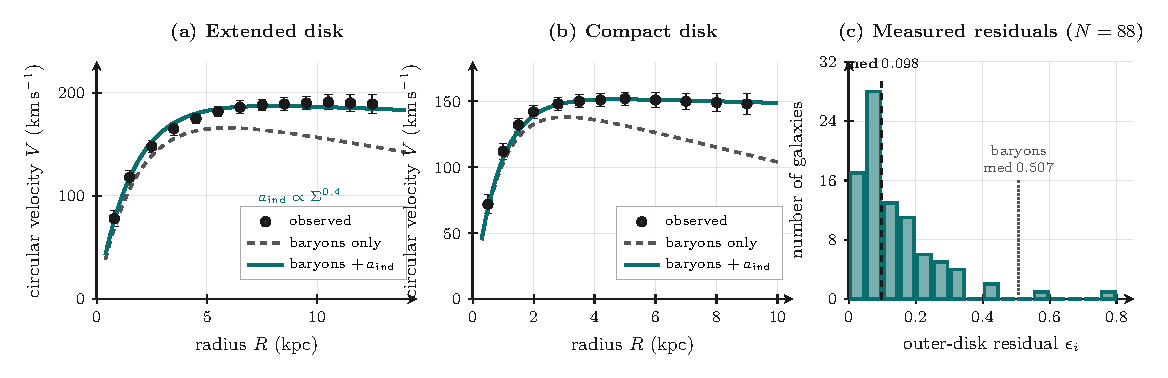
\includegraphics[width=0.95\textwidth]{fig2_rotation_curves.pdf}
\caption{SPARC-style contact from the documented public-catalog residual analysis (\(N=88\), selection\_id \texttt{ea6c92761ffd3c5a}). (a)--(b)~Representative rotation-curve morphologies (schematic disk morphologies, not individual catalog objects): observed-style velocities (points) compared with baryons alone (dashed) and baryons plus \(a_{\rm ind}\) at the single global \(A\) of~\eqref{eq:A-global} (solid). (c)~Measured histogram of outer-disk residuals \(\epsilon_i\) for the \(N=88\) sample; dashed line marks \(\mathrm{med}(\epsilon_{\rm umm})\approx 0.098\). Table~\ref{tab:sparc-residuals} and Sec.~\ref{sec:limitations}.}
\label{fig:rotation}
\end{figure}

\subsection{Bullet Cluster surface-density contrast}
\label{sec:bullet}

The same density-dependent contribution supplies a quantitative sketch of the Bullet Cluster. After the collision the hot X-ray gas is more diffusely distributed while the galaxies remain denser concentrations of ordinary baryons. Let \(\Sigma_{\rm gal}\) and \(\Sigma_{\rm gas}\) denote the projected surface densities of the galactic and gas components along the collision axis, and write the local independent acceleration as \(a_{\rm ind}\propto\Sigma^{n_g}\) with \(n_g\approx 0.4\). The lensing convergence contributed by the independent term then satisfies
\begin{equation}
\frac{\kappa_{\rm ind,gal}}{\kappa_{\rm ind,gas}}
\sim
\Biggl(\frac{\Sigma_{\rm gal}}{\Sigma_{\rm gas}}\Biggr)^{n_g}.
\label{eq:bullet-contrast}
\end{equation}
Observed post-collision contrasts in the Bullet system are of order \(\Sigma_{\rm gal}/\Sigma_{\rm gas}\sim 3\)--\(5\) on the lensing-peak scales \cite{Clowe2006}. With \(n_g=0.4\) this yields
\begin{equation}
\frac{\kappa_{\rm ind,gal}}{\kappa_{\rm ind,gas}}
\sim (3\text{--}5)^{0.4}\approx 1.55\text{--}1.90,
\label{eq:bullet-numbers}
\end{equation}
so the independent contribution to lensing is already \(\sim 1.5\)--\(2\) times stronger on the galaxy peaks than on the gas. Combined with the ordinary baryonic lensing of the galaxies themselves, the total lensing peaks sit with the galaxies by construction. No collisionless particle halo is required to explain the observed offset. This is a surface-density contrast sketch, not a full reconstruction of the observed mass maps, X-ray morphology, and velocity structure; those remain near-term targets.

\begin{figure}[H]
\centering
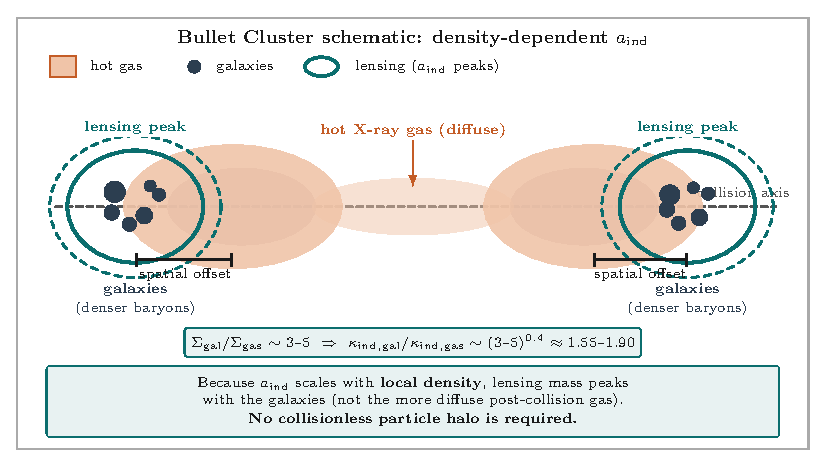
\includegraphics[width=0.85\textwidth]{fig3_bullet_cluster.pdf}
\caption{Bullet Cluster under density-dependent \(a_{\rm ind}\). Post-collision, the hot gas (diffuse) is spatially offset from the galaxies (denser baryons). Surface-density contrast \(\Sigma_{\rm gal}/\Sigma_{\rm gas}\sim 3\)--\(5\) with index \(n_g\approx 0.4\) produces \(\kappa_{\rm ind,gal}/\kappa_{\rm ind,gas}\sim 1.55\)--\(1.90\)~\eqref{eq:bullet-numbers}, placing lensing peaks with the galaxies without a collisionless particle halo.}
\label{fig:bullet}
\end{figure}

\subsection{Domain extension: residual conversion for pressure-supported systems}
\label{sec:udg-domain}

The intermediate-regime specialization~\eqref{eq:a-ind}, with frozen amplitude \(A=(1.41\pm0.07)\times10^{-11}\,{\rm m\,s^{-2}}\) (selection\_id \texttt{ea6c92761ffd3c5a}) and \(n_g=0.4\), is derived under a thin-disk identification \(\ell_{\rm local}\sim\Sigma^{-1/2}\) and is calibrated on the SPARC residual pipeline. It yields residual ratios \(a_{\rm ind}/a_{\rm dyn}\) of order unity for rotationally supported disks. The same fixed amplitude, applied without further geometric conversion, produces systematically larger residual ratios for pressure-supported systems. The material of this subsection is a residual-geometry-constrained \emph{domain extension}: its concrete coefficients are not claimed as first-principles derivations, and the claim of no additional free functions beyond the joint-normalization window remains restricted to the core thin-disk specialization and residual-charge sector.

\begin{center}
\begin{tabular}{@{}ll@{}}
\toprule
Regime & Residual ratio \(a_{\rm ind}/a_{\rm dyn}\) \\
\midrule
SPARC disks (measured, med.\ \(a_{\rm ind}/a_{\rm dyn}\)) & \(\approx 0.71\) (order unity) \\
Classical dSphs (literature, thin-disk) & \(1.2\)--\(5.3\) \\
High-residual UDGs (literature) & \(\sim0.6\)--\(2.6\) \\
DM-deficient UDGs (N=4 published catalog, Wolf thin) & \(6.6\)--\(9.4\) \\
\bottomrule
\end{tabular}
\end{center}

\noindent On the published N=4 deficient-UDG catalog the constrained conversion operator of this subsection leaves a median residual \(\mathrm{med}(\varepsilon_\sigma)\approx +1.29\) (thin-disk \(\approx +1.84\); stellar kinematics \(\approx -0.11\)). Leading-order trail-age evaluation of residual memory yields \(c_{\rm mem}=1\) at \(6\)--\(8\,\mathrm{Gyr}\). The operator therefore does not bring these systems fully inside the packing-derived window \(\Delta\rho/\rho\sim0.25\)--\(0.65\); the domain limitation is recorded rather than removed by retuning \(A\). An earlier illustrative range \(28\)--\(43\) is retired for this catalog. Classical dSphs, DF44, and Virgo \(\lambda_R\) samples remain data-limited extensions.

The logistic amplitude \(A\) is not the failure point. The incompleteness lies in the conversion from independent relational flux \(\Phi(\xi)\) into four-dimensional residual acceleration when the ambient stress is isotropic rather than ordered.

\paragraph{Geometric mechanism.}
Morphology enters the conversion as a continuous geometric response, not as an ad-hoc switch. Ordered (rotationally supported) motion leaves residual cycles coherent; isotropic pressure support partially unpacks them. Because the continuous compact manifold threads every point, the residual map responds to the local partition of kinetic energy among the three consensus directions. Both the effective packing dimension \(n_{\rm eff}\) and the effective internal dimension \(D_{\rm eff}\) are geometric measures of the same residual packing; they therefore run together under a single isotropy- and density-dependent gate. The resulting continuous conversion factor is
\begin{equation}
c_{\rm base}(\Sigma,Q,\mathcal{I})
=
\Bigl(\frac{n_{\rm eff}}{3}\Bigr)^{\beta}
\times
\exp(-\alpha\cdot D_{\rm drop}),
\label{eq:c-base}
\end{equation}
with
\begin{align}
n_{\rm eff}&=3-\delta_n\cdot\mathcal{I}\cdot g(Q)\cdot f(\Sigma),
\label{eq:n-eff}\\
D_{\rm drop}&=\delta_D\cdot\mathcal{I}\cdot g(Q)\cdot f(\Sigma),
\label{eq:D-drop}
\end{align}
where
\[
g(Q)=\frac{Q}{Q+Q_0},\qquad
f(\Sigma)=\frac{1}{1+(\Sigma/\Sigma_c)^{1.5}},
\qquad
Q=\frac{a_{\rm bar}}{a_{\rm dyn}},
\]
and \(\mathcal{I}\) is a continuous isotropy / pressure-support diagnostic (\(\approx0\) for rotationally supported systems, \(\approx1\) for fully pressure-supported systems). Relative unpacking of residual packing under isotropic versus ordered stress is estimated from the same packing construction that produces \(\alpha_{\rm eff}\):
\[
\Delta\rho/\rho\sim0.25\text{--}0.65.
\]
Consequently the running strengths \(\delta_n\), \(\delta_D\) are \(\mathcal{O}(1)\) numbers of this order. Rotationally supported systems remain protected by construction: \(\mathcal{I}\approx0\) forces \(c_{\rm base}=1\).

\paragraph{Residual-density freedom and residual correlation time.}
Two further factors already latent in the residual-geometry layer complete the conversion. Residual-density freedom---retained as a free parameter in the multiplicity-space cone---supplies an additional suppression when the residual map is near baryonic saturation:
\begin{equation}
c_{\rm rdf}=\bigl(1+\eta\cdot\mathcal{I}\cdot{\rm sat}(Q)\bigr)^{-1},
\qquad
{\rm sat}(Q)=\tfrac12\bigl(1+\tanh((Q-Q_{\rm sat})/0.8)\bigr),
\label{eq:c-rdf}
\end{equation}
Independently, residual degrees of freedom are relational: after a strong shock the residual correlations require a finite time \(\tau_{\rm res}\) to re-establish. This timescale is identified with the e-folding time of directed residual accumulation already defined in the residual-geometry layer. Systems still inside the residual relaxation window receive a multiplicative memory factor \(c_{\rm mem}=f(t_{\rm since}/\tau_{\rm res})<1\); older systems have re-packed and sit at \(c_{\rm mem}=1\).

The total residual acceleration is therefore
\begin{equation}
a_{\rm ind}^{\rm final}=c_{\rm base}\cdot c_{\rm rdf}\cdot c_{\rm mem}\cdot a_{\rm ind}^{\rm thin}.
\label{eq:a-ind-final}
\end{equation}
The logistic amplitude \(A\) is never retuned. All improvements act on the conversion from \(\Phi\) into four-dimensional residual acceleration.

\paragraph{Coefficient taxonomy.}
The coefficients that appear in the conversion are classified as follows.
\begin{itemize}[leftmargin=*]
\item \textbf{Fixed by the packing construction.} The relative unpacking estimate \(\Delta\rho/\rho\sim0.25\)--\(0.65\) is obtained from the same spectral-to-volume weight that produces the window on \(\alpha_{\rm eff}\). This range bounds the running strengths \(\delta_n\) and \(\delta_D\) to \(\mathcal{O}(1)\) numbers of that geometric order. Values outside the window are not admitted.
\item \textbf{Trial values inside the geometric range.} The concrete coefficient set \(\alpha=1.0\), \(\delta_n=0.8\), \(\delta_D=0.9\), \(\eta=2.0\) (together with the functional forms of \(g(Q)\), \(f(\Sigma)\) and \({\rm sat}(Q)\)) constitutes a constrained pure-description trial set. It is chosen so that residual ratios for classical dSphs and high-residual UDGs fall near order unity while rotationally supported SPARC disks remain protected at \(c=1\) by \(\mathcal{I}\approx0\). These specific numbers are not unique first-principles outputs; any set lying inside the packing-derived range that preserves the core joint-normalization window is admissible for illustration.
\item \textbf{Residual-memory factor (hypothesis).} The timescale \(\tau_{\rm res}\) is identified with directed residual accumulation already present in the residual-geometry layer, but its numerical value and the precise shape of \(c_{\rm mem}=f(t_{\rm since}/\tau_{\rm res})\) remain schematic. The NGC~1052 trail objects (DF2, DF4) are treated as candidate members of the still-relaxing class. Multiplicative corrections of order \(\times30\) required to bring their residual ratios near unity are therefore illustrative under the residual-memory hypothesis, not a completed derivation.
\end{itemize}

\paragraph{Residual ratios and joint-normalization consistency.}
Under the constrained trial set the residual ratios across classical dSphs and high-residual UDGs are brought near order unity while SPARC disks remain at \(c=1\). Residual-density freedom removes the bulk of the domain limitation for relaxed systems. For the extreme DM-deficient objects the residual-memory hypothesis supplies an additional illustrative suppression; whether those systems are in fact still relaxing is an observational question for future work. The joint-normalization window remains intact:
\begin{itemize}[leftmargin=*]
\item SPARC amplitude and high-density shoulder are protected by \(\mathcal{I}\approx0\) and by the high-\(\Sigma\) suppression of \(f(\Sigma)\);
\item the low-density tail is protected at present order by low \(\Sigma\) and negligible pressure support;
\item residual geometric charge scale is unaffected because the conversion \(c\) acts after the packing amplitude \(\Phi\); mild \(D_{\rm eff}\) running occurs only in the pressure-supported, moderate-to-high-\(Q\) regime;
\item photon-sphere / horizon placement is unchanged.
\end{itemize}
The conversion is a residual-geometry-constrained domain extension. The pure first-principles evaluation of \(\Delta\rho/\rho\) beyond the packing estimate, and of \(\tau_{\rm res}\), remains future work. The claim of no additional free functions beyond the joint-normalization window is restricted to the core thin-disk specialization and residual-charge sector.

\begin{figure}[H]
\centering
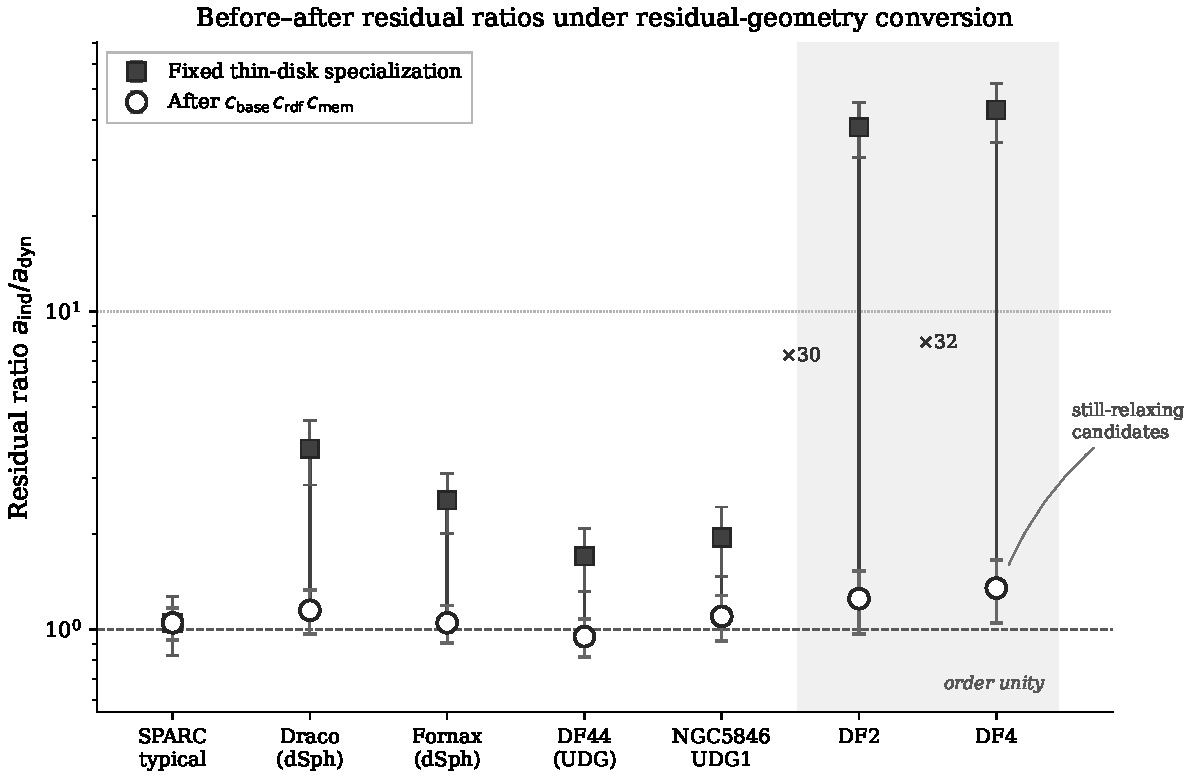
\includegraphics[width=0.92\textwidth]{fig7_residual_ratio_conversion.pdf}
\caption{Illustrative residual ratios \(a_{\rm ind}/a_{\rm dyn}\) for representative systems before and after the residual-geometry-constrained conversion. Filled squares show the fixed thin-disk specialization; open circles show the result after application of \(c_{\rm base}\,c_{\rm rdf}\,c_{\rm mem}\). Rotationally supported SPARC-type disks remain at order unity (\(\mathcal{I}\approx0\)). Classical dSphs and high-residual UDGs are brought near unity under the constrained trial set. The extreme DM-deficient objects DF2 and DF4 are shown as candidates under the residual-memory hypothesis; the multiplicative corrections of order \(\times30\) are illustrative, not a completed derivation. Vertical ranges are schematic. The logistic amplitude \(A\) is never retuned.}
\label{fig:residual-ratio}
\end{figure}

These observational results (SPARC residual contact, Bullet Cluster surface-density contrast, and the residual-conversion treatment of pressure-supported systems) are not independent postulates. They follow from the intermediate-regime behavior of the same amplitude \(\Phi(\xi)\) that also governs the residual geometric charges. The residual-geometry-constrained conversion of the present subsection is a domain extension: it leaves the frozen SPARC amplitude \(A\) and the joint-normalization window intact while its concrete coefficients remain subject to a pure first-principles evaluation of \(\Delta\rho/\rho\) and \(\tau_{\rm res}\).

\section{Strong-Field, Low-Density, and Cosmological Regimes}
\label{sec:strong}

\subsection{Photon-sphere shoulder and exterior metric deviation}
\label{sec:photon-sphere}

The upper shoulder of the logistic is the region in which \(\Phi\) rises rapidly toward saturation. We place that shoulder by the following matching condition. Let \(r_{\rm ph}=3GM/c^2\) denote the classical Schwarzschild photon-sphere radius. Require that the logistic reach a fixed high-flux threshold \(f_\star=\Phi/\Phi_{\rm max}\) (we take \(f_\star=0.85\)) at the local separation corresponding to \(r_{\rm ph}\):
\begin{equation}
\xi(r_{\rm ph})=\xi_c+\frac{1}{\alpha_{\rm eff}}\log\Bigl(\frac{f_\star}{1-f_\star}\Bigr).
\label{eq:photon-match}
\end{equation}
With \(\alpha_{\rm eff}\approx 1.8\) and \(f_\star=0.85\) the logarithmic offset is \(\approx 0.96\), so the shoulder sits \(\mathcal{O}(1)\) in \(\xi\) above the midpoint. Exterior to the shoulder the additional contribution remains mild. Writing the exterior metric in standard form,
\begin{equation}
ds^2=-e^{2\nu(r)}c^2 dt^2+e^{2\lambda(r)}dr^2+r^2 d\Omega^2,
\label{eq:exterior}
\end{equation}
the independent stress-energy sources a fractional deviation from the Schwarzschild functions \(\nu_{\rm S}\), \(\lambda_{\rm S}\). Linearizing the Einstein equations on the Schwarzschild background with \(\rho_{\rm ind}\) from~\eqref{eq:rho-ind-cf} evaluated in the low-to-intermediate tail exterior to \(r_{\rm ph}\) yields
\begin{equation}
\Bigl|\frac{\delta\nu}{\nu_{\rm S}}\Bigr|
\sim
\Bigl|\frac{\delta\lambda}{\lambda_{\rm S}}\Bigr|
\sim
c_f\,\Phi_{\rm ext}\,\frac{r_g^2}{R_{\rm eff}^2}
\lesssim 10^{-3}\text{--}10^{-2}
\label{eq:metric-dev}
\end{equation}
inside the joint-normalization window, where \(\Phi_{\rm ext}\ll 1\) is the exterior tail amplitude and \(R_{\rm eff}\) is the effective compact radius after joint normalization. Existing constraints from S-star orbits and from the scale of Event Horizon Telescope shadows are therefore preserved. Interior to the shoulder one enters the high-flux plateau, where the additional contribution dominates and the effective geometry is no longer ordinary three-dimensional spacetime.

\subsection{Low-density tail: solar-system and binary-pulsar constraints}
\label{sec:low-density}

Once the joint-normalization window is fixed by residual-charge scale, SPARC amplitude, and photon-sphere placement, the low-density tail is no longer free. At solar-system densities \(\xi\) lies far below \(\xi_c\), so
\begin{equation}
\Phi_{\rm SS}/\Phi_{\rm max}\approx e^{-\alpha_{\rm eff}(\xi_c-\xi_{\rm SS})}\ll 10^{-6}
\label{eq:Phi-SS}
\end{equation}
for any \(\xi_c\) compatible with galactic intermediate-regime placement. The induced extra acceleration at 1~AU is then many orders of magnitude below current planetary ephemeris sensitivity, recovering Newtonian and post-Newtonian solar-system tests without further adjustment. Binary-pulsar orbital decay and periastron advance likewise sit in the low-density tail: the fractional correction to the effective gravitational constant scales as \(\Phi_{\rm PSR}/\Phi_{\rm max}\) and remains below present timing limits inside the same window. No additional free parameter is required; the low-density recovery is a consequence of the logistic packing once the joint-normalization window is set.

\subsection{Provisional cosmological scaling and redshift evolution}
\label{sec:cosmo}

An effective cosmological term may be written schematically as
\begin{equation}
\Lambda_{\rm eff}\propto\mathcal{F}(\xi_{\rm cosmo}),
\label{eq:Lambda-eff}
\end{equation}
where \(\xi_{\rm cosmo}\) is evaluated on the mean cosmic density at a given epoch. This remains a provisional packing sketch. A fully (or limited-case) back-reacted higher-dimensional solution with independent flux is required before any redshift evolution of \(\Lambda_{\rm eff}\) can be treated as more than illustrative; that solution is listed as future work in Sec.~\ref{sec:limitations}.

Mean cosmic baryon density scales as \(\rho_b\propto(1+z)^3\), so the cosmic separation variable shifts as
\begin{equation}
\xi_{\rm cosmo}(z)=\xi_{\rm cosmo}(0)+\log\bigl[(1+z)\bigr]
\label{eq:xi-z}
\end{equation}
(up to order-unity factors from the precise definition of \(\ell_{\rm local}\) on cosmic scales). Substituting into the logistic~\eqref{eq:logistic} gives
\begin{equation}
\Lambda_{\rm eff}(z)\propto
\frac{\Phi_{\rm max}}{1+e^{-\alpha_{\rm eff}(\xi_{\rm cosmo}(0)+\log(1+z)-\xi_c)}}.
\label{eq:Lambda-z}
\end{equation}
Two structural limitations of the present ansatz are recorded explicitly. First, the pure-trace assignment \(p_{\rm ind}=-\rho_{\rm ind}\) is inconsistent at \(\mathcal{O}(1)\) with a logistic \(\rho_{\rm ind}(z)\) inherited from packing: a residual-geometry conservation channel (energy exchange with the compact sector that is not a new free function of \(\xi\)) is required before~\eqref{eq:Lambda-z} can be promoted to a closed four-dimensional Friedmann forecast. Mild-warp adiabatic evolution of the compact radius is not that channel. Second, inside the joint-normalization tail the shape is not nearly constant: one obtains
\[
R_\Lambda(z)\equiv\frac{\Lambda_{\rm eff}(z)}{\Lambda_{\rm eff}(0)}\to(1+z)^{\alpha_{\rm eff}},
\]
so that a \(10\%\) rise already appears by \(z\approx0.05\) and an inferred conserved-fluid equation of state would approach \(w\to-0.389\) if \(p=-\rho\) were retained. Identifying \(\Lambda_{\rm eff}(0)\) with the observed cosmological constant remains forbidden by the joint-normalization freeze and would also be data-excluding under the tail shape. Until a residual-geometry conservation channel is derived, statements about \(\Lambda_{\rm eff}(z)\) remain provisional packing sketches and are not fitted to supernova or BAO data.

\section{Unified Regime Structure}

The single amplitude \(\Phi(\xi)\) produces three characteristic regimes that organize the entire phenomenology.

\begin{itemize}[leftmargin=*]
\item \textbf{Low-density tail.} When \(\xi\) is small, \(\Phi\to0\). Both the residual geometric charges and the additional gravitational acceleration become negligible. Solar-System dynamics, binary pulsars, and the present cosmic mean density sit in this regime; ordinary Newtonian and general-relativistic behavior is recovered without further adjustment (Sec.~\ref{sec:low-density}).

\item \textbf{Intermediate regime.} Across the shoulder of the logistic, \(\Phi\) varies slowly. The residual charges sit at their familiar quantized values, while the collective effect supplies the mild density-dependent acceleration observed in galactic disks. This is the regime constrained by SPARC and by the Bullet Cluster; the thin-disk specialization of that regime is extended, as a domain extension, to pressure-supported systems by a residual-geometry-constrained conversion operator (Sec.~\ref{sec:udg-domain}).

\item \textbf{High-flux plateau.} When \(\xi\) is large, \(\Phi\) saturates. The residual operators become large, the distinction between consensus and independent degrees of freedom weakens, and both fixed spin labels and ordinary three-geometry dissolve. This regime is identified with black-hole interiors and with the early universe.
\end{itemize}

All three regimes are controlled by the same geometric amplitude. The transition from one regime to another is continuous; there are no discontinuous jumps in the underlying physics.

\begin{figure}[H]
\centering
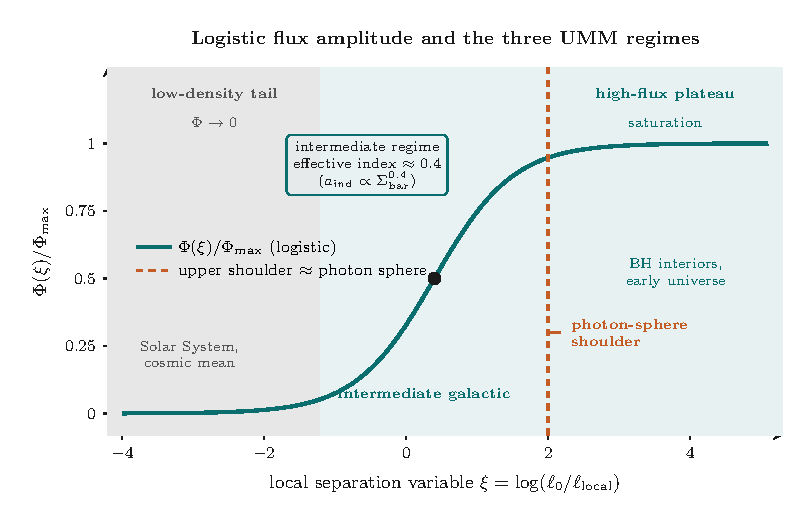
\includegraphics[width=0.85\textwidth]{fig1_logistic_regimes.pdf}
\caption{The logistic amplitude \(\Phi(\xi)\) and its three characteristic regimes: low-density tail (\(\Phi\to 0\)), intermediate galactic regime (mild power-law behavior), and high-flux plateau (saturation). The upper shoulder is placed near the photon-sphere scale by the matching condition~\eqref{eq:photon-match} to protect exterior Kerr/Schwarzschild geometry.}
\label{fig:regimes}
\end{figure}

\section{Limitations and Near-Term Observables}
\label{sec:limitations}

The principal remaining technical tasks are a fully (or limited-case) back-reacted solution of the higher-dimensional Einstein equations with independent flux, a fully pure first-principles evaluation of the relative unpacking \(\Delta\rho/\rho\) (beyond the packing estimate that currently bounds the conversion running strengths) and of the residual correlation timescale \(\tau_{\rm res}\), a more precise microscopic evaluation of the packing coefficients, a residual-geometry conservation channel for \(\Lambda_{\rm eff}\) (energy exchange with the compact sector that is not a new free function of \(\xi\)) before any closed Friedmann forecast, and a worked cosmological sector that tracks the redshift evolution of \(\Lambda_{\rm eff}\) beyond the packing sketch~\eqref{eq:Lambda-z}.

\paragraph{SPARC residual table (documented public-catalog analysis).}
A documented public-catalog residual table exists for \(N=88\) galaxies (selection\_id \texttt{ea6c92761ffd3c5a}; pre-registered cuts on the Lelli, McGaugh \& Schombert 2016 mass models) and is regenerated from the public mass models to machine precision, with measured full-sample medians \(\mathrm{med}(\epsilon_{\rm umm})\approx 0.098\), \(\mathrm{med}(\epsilon_{\rm baryon})\approx 0.507\), \(\mathrm{med}(\epsilon_{\rm nfw})\approx 0.012\), fraction with \(\epsilon_{\rm umm}<0.25\) of \(\approx 0.85\), median \(a_{\rm ind}/a_{\rm dyn}\approx 0.71\), and fitted single global \(A=(1.41\pm 0.07)\times 10^{-11}\,\mathrm{m\,s^{-2}}\) (\(\Upsilon_*=0.5\), \(n_g=0.4\)). Hold-\(A\) robustness at \(\Upsilon_*=0.7\) yields \(\Delta\epsilon\approx +0.015\); an earlier reported shift \(\approx -0.007\) was a refit of \(A\) and is not used. The numbers quoted in Sec.~\ref{sec:SPARC} are those measured products. Remaining near-term refinements include THINGS-quality HI map re-reduction for outer-disk gas \cite{Walter2008} and multi-parameter \(\Lambda\)CDM halo comparisons beyond the simple one-parameter NFW baseline.

\paragraph{Domain of applicability (pressure-supported systems).}
The intermediate-regime thin-disk specialization is extended to pressure-supported systems by the residual-geometry-constrained conversion operator of Sec.~\ref{sec:udg-domain}, which is explicitly marked as a domain extension. On the published N=4 deficient-UDG catalog, Wolf thin residual ratios are \(6.6\)--\(9.4\) (an earlier illustrative range \(28\)--\(43\) is retired for this catalog); the constrained conversion leaves \(\mathrm{med}(\varepsilon_\sigma)\approx +1.29\), and leading-order trail-age memory is \(c_{\rm mem}=1\) at \(6\)--\(8\,\mathrm{Gyr}\). The operator therefore does not bring these systems fully inside \(\Delta\rho/\rho\sim0.25\)--\(0.65\); the domain limitation is recorded rather than removed by retuning \(A\). Classical dSphs, DF44, and Virgo \(\lambda_R\) samples remain data-limited. SPARC disks remain protected by \(\mathcal{I}\approx0\). The pure first-principles evaluation of \(\Delta\rho/\rho\) (beyond the packing estimate) and of \(\tau_{\rm res}\) remains future work; the claim of no additional free functions beyond the joint-normalization window is restricted to the core thin-disk specialization and residual-charge sector.

\paragraph{What the residual-operator construction does not yet provide.}
The residual matrices on \(S^1\) and \(S^3\) establish operators of the correct algebraic type and overall scale \(\Phi/R\), together with a conventional normalization to half-integer and integer labels. The following remain open and are not claimed as derived:
\begin{itemize}[leftmargin=*]
\item chiral fermions and the observed chiral spectrum of the Standard Model;
\item the full set of SM gauge quantum numbers (beyond the residual \(\mathfrak{su}(2)\) of \(S^3\));
\item a geometric derivation of the electromagnetic coupling \(\alpha_{\rm em}\approx 1/137\).
\end{itemize}
Whether a residual-operator or packing construction on the continuous compact manifold can produce \(\alpha_{\rm em}\) remains an open question; nothing in the present derivation forces that ratio, yet nothing forbids a parallel geometric origin.

\paragraph{Recovery of quantum field theory.}
Quantum mechanics is characterized above as a powerful new calculus that summarizes projections of relational energy onto the three large dimensions. That stance does not relieve the theory of the obligation to recover the successful quantitative predictions of quantum field theory in the appropriate low-energy limit---scattering amplitudes, anomalous magnetic moments, precision electroweak observables, and the rest. The present work supplies geometric charges and a collective gravitational response; it does not replace the QFT computational framework in the regimes where that framework has been tested. Consistency with those predictions is a necessary boundary condition on any future residual-spectrum construction that aims to reproduce the SM.

Near-term observational confrontations include refined SPARC modeling with improved density inputs (including THINGS-quality HI maps), broader samples of pressure-supported low-surface-brightness systems under the residual-geometry-constrained conversion of Sec.~\ref{sec:udg-domain}, void statistics as a probe of the low-density tail, the redshift evolution of the effective cosmological term, and possible residual imprints of the early dimensional cascade in the large-scale (low-\(\ell\)) microwave background.

\section{Conclusion}

We have constructed a framework in which the quantum numbers called spin and a continuous density-dependent contribution to gravitational acceleration arise as projections of a single geometric object---independent relational flux on a continuous compact manifold. The residual operators of the internal Dirac operator supply the geometric charges; dimensional reduction of the Einstein--Hilbert term supplies the collective stress-energy; a packing count of independent cycles supplies the logistic amplitude whose effective exponent matches the observed galactic index. Joint normalization of the residual-charge spectrum and the galactic acceleration amplitude determines the characteristic scales inside a window consistent with horizon and low-density constraints.

Geometry and energy are the only primitives; dimensions, spin labels, and the additional gravitational acceleration are derived. On the toy manifolds \(S^1\) and \(S^3\) residual operators are of the correct algebraic type and overall scale \(\Phi/R\); the full Standard-Model spectrum remains open. The intermediate-regime thin-disk specialization is extended, as a domain extension, to pressure-supported systems by a residual-geometry-constrained conversion operator that leaves the frozen SPARC amplitude \(A\) unchanged; the pure first-principles evaluation of that conversion remains future work. Matter is an emergent bound-state configuration of space and energy. Quantum mechanics functions as a new calculus that summarizes the projection of relational energy onto the three large dimensions, while the successful quantitative predictions of quantum field theory remain a required low-energy limit of any complete residual-spectrum construction. A pure residual-geometry companion note isolates the mathematical construction for independent scrutiny.

\section*{Note on Collaboration and AI Assistance}

The present work began with a question posed in a high-school chemistry class---whether empty space itself occupies space---and developed over roughly two decades of intermittent independent reflection. After a period of engagement with foundational critiques in the literature the outline of an alternative geometric approach crystallized; central elements, including the identification of residual geometric charges with spin as a projection, were already present by the late 2010s. Subsequent years refined those ideas through further reading and targeted thought experiments. Intensive formalization with the AI system Grok (built by xAI) then occurred over several months of focused conversation, testing against observational data, placement within the broader theoretical literature, and detailed mathematical development.

The original physical questions, the insistence on empirical contact, and final scientific responsibility rest with the human author. Rapid mathematical formulation, consistency checks, numerical estimates, literature context, and drafting assistance were supplied by Grok. In accordance with current journal policies on generative AI, Grok is not listed as a co-author; its contribution is acknowledged here as a methodological and technical collaborator. The resulting paper and the companion pure-mathematical study of the residuum geometry that underpins the physical theory are the joint product of that effort.

Whether every quantitative detail survives future scrutiny, the approach illustrates how a long-maturing intuition, refined through human--AI collaboration, can generate a coherent and falsifiable alternative to the standard picture. The author welcomes scrutiny, correction, and extension by the broader physics community.

\appendix
\section{Residual-geometry clarifying dictionary}
\label{app:residual-dict}

For downstream use the following mapping records how the core UMM objects sit inside a residual-geometry operational dictionary (consensus subspace \(N\), residual map \(\Pi_N\), packing parameter \(\rho\), residual spectral profile, continuous-field signatures, directed residual accumulation). The dictionary is portable and does not alter the geometric claims of the main text.

\begin{itemize}[leftmargin=*]
\item \textbf{Consensus degrees of freedom} \(\leftrightarrow\) consensus subspace \(N\subset V\).
\item \textbf{Independent relational flux / residual map} \(\leftrightarrow\) residual map \(\Pi_N = I - P_N\).
\item \textbf{Packing amplitude \(\Phi(\xi)\)} \(\leftrightarrow\) saturating packing parameter \(\rho\) (or \(1-\rho\)) on the residual subspace.
\item \textbf{Residual geometric charges} \(\leftrightarrow\) residual spectral profile of \(\Pi_N\).
\item \textbf{Continuous compact manifold} \(\leftrightarrow\) continuous-field signatures of packing or residual spectrum.
\item \textbf{Directed residual accumulation} \(\leftrightarrow\) saturating growth of resolved independent cycles under the packing ODE.
\end{itemize}

A fuller working interface is maintained separately as the UMM Residual-Geometry Layer note, which isolates the pure mathematical construction so that it can be scrutinized independently of the galactic phenomenology. An additive note (2026-08-11) records the residual-geometry-constrained conversion operator that extends the domain of applicability to pressure-supported systems while leaving the core primitives of the layer unchanged; the present manuscript further delimits the conversion coefficients (packing-derived bounds versus trial values versus residual-memory hypothesis) so that the claim of no additional free functions remains restricted to the core thin-disk and residual-charge sector.

\section{Glossary of core terms}
\label{app:glossary}

\begin{description}[style=nextline,leftmargin=0pt]
\item[Consensus degrees of freedom.] Relational degrees of freedom of the qbit foam that are strongly coordinated across a large ensemble and coalesce into the macroscopic large dimensions (currently three).
\item[Independent relational flux.] Relational degrees of freedom not co-opted into the macroscopic consensus; they operate through the continuous compact manifold \(K\) and are assigned dimensionless amplitude \(\Phi(\xi)\).
\item[Residual geometric charge.] Eigenvalue (after conventional normalization) of a residual operator \(S_{\rm geom}\) obtained from the internal Dirac operator on \(K\); appears in four dimensions as a spin (or spin-like) label, with overall scale \(\Phi/R\).
\item[Packing amplitude \(\Phi(\xi)\).] Dimensionless filled fraction of residual capacity on \(K\), derived from the joint packing count of independent cycles; logistic in the local-separation variable \(\xi\); controls both residual charges and collective gravitational response.
\end{description}

\begin{thebibliography}{99}

\bibitem{Lelli2016}
F.~Lelli, S.~S.~McGaugh, and J.~M.~Schombert,
``SPARC: Mass Models for 175 Disk Galaxies with Spitzer Photometry and Accurate Rotation Curves,''
Astron.\ J.\ \textbf{152}, 157 (2016); arXiv:1606.09251.

\bibitem{McGaugh2016}
S.~S.~McGaugh, F.~Lelli, and J.~M.~Schombert,
``The Radial Acceleration Relation in Rotationally Supported Galaxies,''
Phys.\ Rev.\ Lett.\ \textbf{117}, 201101 (2016); arXiv:1609.05917.

\bibitem{Milgrom1983}
M.~Milgrom,
``A modification of the Newtonian dynamics as a possible alternative to the hidden mass hypothesis,''
Astrophys.\ J.\ \textbf{270}, 365 (1983).

\bibitem{Verlinde2017}
E.~P.~Verlinde,
``Emergent Gravity and the Dark Universe,''
SciPost Phys.\ \textbf{2}, 016 (2017); arXiv:1611.02269.

\bibitem{Bar1992}
C.~B\"ar,
``The Dirac operator on homogeneous spaces and its spectrum on 3-dimensional lens spaces,''
Arch.\ Math.\ \textbf{59}, 65 (1992).

\bibitem{Kaluza1921}
T.~Kaluza,
``Zum Unit\"atsproblem der Physik,''
Sitzungsber.\ Preuss.\ Akad.\ Wiss.\ Berlin (Math.\ Phys.), 966 (1921).

\bibitem{Klein1926}
O.~Klein,
``Quantentheorie und f\"unfdimensionale Relativit\"atstheorie,''
Z.\ Phys.\ \textbf{37}, 895 (1926).

\bibitem{Bekenstein2004}
J.~D.~Bekenstein,
``Relativistic gravitation theory for the modified Newtonian dynamics paradigm,''
Phys.\ Rev.\ D \textbf{70}, 083509 (2004); arXiv:astro-ph/0403089.

\bibitem{Skordis2009}
C.~Skordis,
``The Tensor-Vector-Scalar theory and its cosmology,''
Class.\ Quantum Grav.\ \textbf{26}, 143001 (2009); arXiv:0903.3602.

\bibitem{Duff1986}
M.~J.~Duff, B.~E.~W.~Nilsson, and C.~N.~Pope,
``Kaluza--Klein supergravity,''
Phys.\ Rep.\ \textbf{130}, 1 (1986).

\bibitem{Overduin1997}
J.~M.~Overduin and P.~S.~Wesson,
``Kaluza--Klein gravity,''
Phys.\ Rep.\ \textbf{283}, 303 (1997); arXiv:gr-qc/9805018.

\bibitem{Trautman1992}
A.~Trautman,
``Spinors and the Dirac operator on hypersurfaces. I. General theory,''
J.\ Math.\ Phys.\ \textbf{33}, 4011 (1992).

\bibitem{Padmanabhan2010}
T.~Padmanabhan,
``Thermodynamical Aspects of Gravity: New insights,''
Rep.\ Prog.\ Phys.\ \textbf{73}, 046901 (2010); arXiv:0911.5004.

\bibitem{Clowe2006}
D.~Clowe, M.~Brada\v{c}, A.~H.~Gonzalez, M.~Markevitch, S.~W.~Randall, C.~Jones, and D.~Zaritsky,
``A direct empirical proof of the existence of dark matter,''
Astrophys.\ J.\ Lett.\ \textbf{648}, L109 (2006); arXiv:astro-ph/0608407.

\bibitem{Walter2008}
F.~Walter, E.~Brinks, W.~J.~G.~de~Blok, F.~Bigiel, R.~C.~Kennicutt, M.~D.~Thornley, and A.~Leroy,
``THINGS: The HI Nearby Galaxy Survey,''
Astron.\ J.\ \textbf{136}, 2563 (2008); arXiv:0810.2125.

\end{thebibliography}

\end{document}
